\documentclass[format=acmsmall, review=false]{acmart}
\settopmatter{printacmref=false, printccs=false}
\usepackage{booktabs} % For formal tables
\usepackage[ruled]{algorithm2e} % For algorithms
\usepackage{enumitem}
\usepackage{subcaption}
\newcommand{\xhdr}[1]{\vspace{1mm} \noindent{\bf #1}}
\renewcommand{\footnotetextcopyrightpermission}[1]{} % remove copyright block
\renewcommand{\footnotetextauthorsaddresses}[1]{} % remove author address 
\renewcommand{\algorithmcfname}{ALGORITHM}
\SetAlFnt{\small}
\SetAlCapFnt{\small}
\SetAlCapNameFnt{\small}
\SetAlCapHSkip{0pt}
\IncMargin{-\parindent}

% Choose a citation style by commenting/uncommenting the appropriate line:
%\setcitestyle{authoryear}
\setcitestyle{acmnumeric}

\newtheorem{finding}{Finding}

% Title. Note the optional short title for running heads. In the interest of anonymization, please do not include any acknowledgements.
\newcommand\PaperTitle{Deconstructing the Filter Bubble: \\ Consumer Decision-Making and Recommender Systems}
\title[\PaperTitle]{\PaperTitle}

% Anonymized submission.

% Abstract. Note that this must come before \maketitle.
\begin{abstract}
We study a model of user decision-making in the context of recommender systems via numerical simulation. Our model provides an explanation for the findings of Nguyen, et. al (2014), where users consume increasingly similar items over time even without recommendation. Our model naturally generates such filter bubble effects since users face a sequential decision making problem under uncertainty and there are informational spillovers where a user consuming a item and learning how she values it reduces uncertainty and provides information about similar items. As shown in Nguyen, et. al (2014), recommendation alleviates these filter bubble effects and we further find that, by providing users with information, recommendation leads users to consume increasingly similar items. Finally, our model highlights the importance of collecting data on user beliefs and their evolution over time both to design better recommendations and to further understand their impact.
\end{abstract}

\begin{document}

\maketitle


% Paper body
\section{Introduction}

Recommender Systems (RS) have become critical for assisting users in navigating the large choice sets that they face in many online platforms. For instance, users have to select from thousands of movies on Netflix, millions of products on Amazon, and billions of videos on YouTube. Users in many cases are not aware of most items, let alone have full information about their preferences over them. To make matters worse, the item in these contexts are usually experience goods whose true value can only be learned after consumption.
\par

Recommender systems have been influential in shaping consumer choice in these markets with 75\% of movies watched on Netflix and 35\% of page-views on Amazon coming from recommendations.\footnote{MacKenzie et al. (2013, Oct.),  How retailers can keep up with consumers. \url{https://www.mckinsey.com/industries/retail/our-insights/how-retailers-can-keep-up-with-consumers}. Retrieved on October 3, 2019.} While there are many positive effects from these systems, there is an increasing worry that there are unintended side-effects of recommendation systems. There have been claims that personalized recommender systems lead users into \textit{filter bubbles} where they effectively get isolated from a diversity of viewpoints or content \cite{pariser2011filter}, and that personalized recommender systems may also lead users to become increasingly homogenized at the same time \cite{chaney2018algorithmic, hosanagar2013will}.
\par
Understanding how recommender systems influence user behavior is important not only for characterizing the broader consequences of such systems but also for guiding their design. In this paper we develop a theoretical model of user decision-making in contexts where recommender systems are traditionally deployed. We utilize previous empirical studies that characterize how recommender systems influence user choice as a benchmark and our theoretical model provides an intuitive mechanism that provides an explanation for these empirical results. The key insight of our model is that individual \textit{beliefs} drive the consumption choices of individuals and that recommendations serve to provide users with information that leads them to update their beliefs. However, a crucial component of our model is that individuals' beliefs about items are driven not only by recommendations, but also from their previous experiences with similar items. We use these insights to provide guidance for recommender system designers. In order to design good recommendations it becomes crucial for designers to understand user beliefs of goods they haven't consumed thus far and how these beliefs evolve over time.

\xhdr{Our Model} We consider a model of user choice that has the following components.
\par
The first component of our model is that users sequentially consume items and face large choice sets. In our setting of interest users are long-lived, but they only consume a small fraction of this choice set over their lifetime. This is traditionally the case on online platforms that have thousands or millions of options for users.
\par
The second component of our model is that users have \textit{uncertainty} about their valuation of the different items before they consume them. This is motivated both by the fact that many contexts where recommender systems are deployed contain experience goods, whose true value can only be learned after consumption, and the fact that such uncertainty is why recommender systems exist in the first place. Thus, users face a sequential decision-making problem under uncertainty.
\par 
The third, and key, component of our model is that consumption of an item reveals information that changes user beliefs about the valuation of similar items. Unlike in standard sequential decision-making problems, in our model once an item is consumed all uncertainty about its valuation is resolved. This valuation provides information for consumers that enables them to update their beliefs about similar items. This exploits the fact that the valuations of similar items are correlated which assists users in navigating the vast product space. The idea that users make similarity-based assessments to guide their choice has grounding in theoretical work in decision theory \cite{gilboa1995case} and empirical evidence of how users navigate large choice sets \cite{schulz2019structured}.
\par 
The fourth component of our model is that recommendation provides users with information about the true valuations. We model the realized valuations as being a weighted sum of a common-value and an idiosyncratic component. This formulation gives a stylized notion of predictability of user preferences where the idiosyncratic component is inherently unpredictable given other individuals' preferences and the common-value component is what the recommender can learn from previous users' data. We suppose that the recommender knows the common-value component for each item and combines it with individuals' beliefs over the product space when designing personalized recommendation.

\xhdr{Our Contributions}
Our model provides a clear mechanism that explains the empirical results in \cite{nguyen2014exploring} who show that, in the context of movie consumption, user behavior is consistent with filter bubble effects even without recommendation and that recommendation leads to users being less likely to fall into such filter bubbles. In this context, filter bubble effects are defined as users consuming items in an increasingly narrow portion of the product space. The simple and intuitive driving force of this in our model is that preferences for similar items are correlated, which implies that when an item is consumed and the user learns its value, it provides information about similar items. Crucially, this not only impacts the underlying belief about the average utility of the item, but also the level of uncertainty. Consequently, this learning spillover induces users to consume items ``similar'' to those they consumed before that had high realized value, leading to an increasing narrowing of consumption patterns towards these regions of the product space. This effect is further amplified when users are \textit{risk-averse}, a concept from decision theory where all else being equal, users have a preference for goods with lower uncertainty to those with higher uncertainty. However, by providing information to users, recommendation leads users to be more likely to explore other portions of the product space, limiting the filter bubble effect.
\par
We find that, while recommendation leads a single user to be more likely to explore diverse portions of the product space, it also coordinates consumption choices across users. This leads to an increase in homogeneity across users, resulting in a tradeoff between homogenizing across user consumption and diversifying within user consumption. We finally explore the relationship between the overall diversity of consumed items and user welfare. We find that more diverse sets of consumed items do not always correspond to higher user welfare. 
\par
Finally, we discuss how our model and findings can be used to inform the design and evaluation of recommender systems as well as the data that is traditionally collected for them. Our model highlights the importance of user beliefs in determining the consumption choices of individuals and how both recommendation and informational spillovers determine how these beliefs change over time. By collecting information on user beliefs, recommender system designers can understand what items a user would consume \textit{without} recommendation and then predict how providing information to the user would change their beliefs and resulting consumption decisions. Thus,  our evaluation measure determines the value of a recommendation based on the marginal welfare gain associated with providing a user with a recommendation over what the user would do without it. We discuss how this provides an additional rationale as to why ``accurate" recommendations are not always good recommendations.
\par

\textbf{Related Work.} 
The first set of related works studies the extent and implications of filter bubbles. \cite{pariser2011filter} first informally described the idea of the ``filter bubble'' which is that online personalization services would lead users down paths of increasingly narrower content so that they would effectively be isolated from a diversity of viewpoints or content. Following this a number of empirical studies, done in various disciplines, have since studied the extent to which this phenomenon exists in a wide range of contexts \cite{flaxman2016filter,hosanagar2013will,moller2018blame,nguyen2014exploring}. The most relevant to our study is \cite{nguyen2014exploring} who study whether this effect exists with recommender systems in the context of movie consumption. They find that even users whose consumption choices are not guided by recommendations fall into behavior consistent with ``filter bubbles'' and that recommender systems can actually increase the diversity of the content that users consume. To our knowledge there are no theoretical models that rationalize these empirical findings and our paper provides a theoretical framework through which to view this problem. Further, our paper provides a clear mechanism at play that drives such effects and how recommendation interacts with them.
\par 
Another set of papers has examined whether recommender systems can lead users to become increasingly homogenized or consume similar content to one another. \cite{celma2008hits, treviranus2009value} show that incorporating content popularity into recommender systems can lead to increased user homogenization. \cite{chaney2018algorithmic} shows how user homogenization may arise from training recommender systems on data from users exposed to algorithmic recommendations. \cite{fleder2009blockbuster} show that homogenization can increase due to a recommendation bias towards popularity that arises from lack of information about items with limited consumption histories. Our model leads to similar results as previous theoretical and empirical work where recommender systems lead to increased user homogenization. However, the mechanisms behind this from our model differ from existing work as homogenization arises due to the fact that recommendation leads users to coordinate their consumption decisions in certain portions of the product space.
\par
Another set of papers studies the impact of human decision-making on the design and evaluation of recommender systems. \cite{chen2013human} surveys the literature on the relationship between human decision making and recommender systems. The closest set of papers pointed out in this survey are those related to preference construction \cite{bettman1998constructive, lichtenstein2006construction} whereby users develop preferences over time through the context of a decision process. Our model points out that the true underlying preferences of users may be stable over time, but, due to the nature of items in contexts where recommender systems are deployed, they have incomplete information of them and both consumption and recommendation provide them with information to reduce their uncertainty. Thus, the primary insight of our paper is that individual beliefs and how individuals update their beliefs about similar items after consumption are important and previously unconsidered elements of human decision making that are critical for understanding the design and consequences of recommender systems. Within this literature, there is a set of papers that focus on ``user-centric" approaches to recommendation \cite{celma2008new, cremonesi2013user, pu2011user} whereby user evaluation of the usefulness of recommendation is a key evaluation measure. Our evaluation measure is similar, but, unlike previous approaches, emphasizes the importance of user beliefs. Finally, \cite{hodgson2019horse} considers a similar model as ours where users engage in ``spatial learning'' and exploit the correlation of their preferences in the environment, but consider it in the context of search for a single item.

\section{Our Model and Preliminaries}
\subsection{Preliminaries on Expected Utility Theory}
\noindent For every item $n$ in the product space $\mathcal J$, we assume that each user $i$ assigns a monetary equivalent $x_{i,n} \in \mathbb R$ to the experience of consuming it. Each user can value the same item differently. However, we assume that users have the same utility over money, given by a utility function $u: \mathbb R \to \mathbb R$, strictly increasing and continuous. So, ex-post, the value of item $n$ for user $i$ is given by $u(x_{i,n})$ However, before consuming the item, the user does not know exactly how she will value it. In particular, even users that will end up having the same ex-post valuation of item $n$ may differ in their ex-ante valuation because they hold different beliefs about it. We denote by $p_{i}$ the beliefs user $i$ has about how she will value each of the items in the product space. Note that this implies that consuming item $n$ is the same as taking a gamble. Each user evaluates the item according to the associated expected utility associated with the item, i.e. $U_i(n)=\mathbb E_{p_i}[u(x_n)]$. 
\par

Risk aversion captures how different users react to the risk associated to a particular consumption opportunity. It is formalized as follows: a given gamble $x$ takes real values and follows distribution $p$. Then, for every gamble $x$, there is a certain amount of money that makes the user indifferent between taking the gamble or taking the sure amount of money. This sure amount of money is called the \textit{certainty equivalent} of gamble $x$ and is denoted as $\delta(x)$. A user $i$ is more risk-averse than another user $j$ when for every gamble $x$, user $i$ requires a lower value to give up the gamble when compared to user $j$, i.e. $\delta_i(x)$. Therefore, a more risk-averse user is more willing to avoid the risk of taking the gamble. We assume that the utility function takes a flexible functional form $u(x)=1-\exp(-\gamma x)$ for $\gamma\ne0$ and $u(x)=x$ for $\gamma=0$ -- known as constant absolute risk-aversion preferences (from hereon CARA). Higher $\gamma$ implies higher risk-aversion with $\gamma=0$ corresponding to the risk-neutral case and $\gamma>0$ to the risk-averse one. Our formulations here follow standard economic decision-theory (see \cite{mas1995microeconomic} for a textbook treatment of these topics).
\par

\subsection{Model}
\par
\xhdr{Users.} We consider a set of users $I$ where each user $i \in I$ faces the same finite set of $N$ items $\mathcal J = \left\{0,1,...,N-1\right\}$. For simplicity, we assume that users only derive pleasure from item $n \in \mathcal{J}$ the first time they consume it.
\par

We denote by $x_{i,n}$ user $i$'s realized value from consuming item $n$. In particular, we consider that the realized value derived from a given item can be decomposed in the following manner: $x_{i,n}= v_{i,n} + \beta v_n$, where $v_{i,n}$ denotes an idiosyncratic component -- i.e. user $i$'s idiosyncratic taste for product $n$ --  and $v_{n}$, a common-value component. One can interpret $v_n$ as a measure of how much item $n$ is valued in society in general and, in a sense, $v_{i,n}$ denotes how $i$ diverges from this overall ranking. The scalar $\beta \in \mathbb{R}_{t}$ denotes the degree to which valuations are idiosyncratic to each user or common across users. If $\beta=0$, it is impossible to generate meaningful predictions of any one's individual preferences based on others, while if $\beta$ is large, every individual has similar preferences.
\par
Stacking values in vector-form, we get the vector of values associated with each item 
$${\left(x_{i,n}\right)}_{n \in \mathcal{J}}=:X_i =V_i+ \beta V $$
where $V_i ={\left(v_{i,n}\right)}_{n \in \mathcal{J}}$ and $V={\left(v_{n}\right)}_{n \in \mathcal{J}}$.
\par
\xhdr{User Decision-Making.}
We assume the user makes $T$ choices and therefore can only consume up to $T$ items, where $T$ is a small fraction of $N$. This captures the idea that users are faced with an immense choice set but that ultimately they end up experiencing (and learning) about just a small fraction of it. Since this is a sequential decision-making problem under uncertainty, in principle users face an exploration-exploitation trade-off. However, for tractability, we impose that users are myopic and every period consume the product that they have not yet tried ($n_i^t$) that gives them the highest expected utility given the information from past consumption offers ($C_i^{t-1}=(n_i^1,...,n_i^{t-1})$) and their initial beliefs.
\par
\xhdr{User Beliefs.} We assume that all the true realized values are drawn at $t = 0$. However, users do not know the realized values before consuming an item, but rather have beliefs over the realized utilities.
Formally, user $i$ starts with some beliefs about $X_i$, namely that the idiosyncratic and common-value parts of the valuations are independent -- $V_i \perp \!\!\! \perp V$ -- and that each is multivariate normal 
\begin{enumerate}[topsep=0pt]
\item $V_i \sim \mathcal N (\overline V_i, \Sigma_i)$ 
\item $V \sim \mathcal N(\overline V, \Sigma)$ with $\overline V =0$
\end{enumerate}
We impose the normality assumption for two reasons. The first is that this allows for simple and tractable belief updating. The second is that it allows us to incorporate an easily interpretable correlation structure between the items. The precise formulation of $\Sigma$ and $\Sigma_i$ that we consider is defined below when we discuss user learning.
\par
Keeping with the assumption that $V_i$ represents idiosyncratic deviations from $V$, we assume that, on the population level, prior beliefs $\overline V_i=\left(\overline v_{i,n}\right)_{n \in \mathcal{J}}$ are drawn independently from a jointly normal distribution, where $\overline v_{i,n} \sim \mathcal N (0, \overline \sigma^2)$ are independent and identically distributed. These $\overline v_{i,n}$ denote the prior belief that individual $i$ holds about her valuation over item $n$. As people are exposed to different backgrounds, their beliefs about how much they value a given item also varies and $\overline v_{i,n}$ denotes this idiosyncrasy at the level of prior beliefs.
\par

We assume users are expected utility maximizers. User $i$'s certainty equivalent for item $n$, the sure value that makes user $i$ indifferent between it and consuming the item $n$, conditional on the consumption history, is given by
$\delta_{i}(n)\mid C_i^{t-1}=\mu_n-\frac{1}{2}\gamma \Sigma_{nn}$, where $\mu_n$ and $\Sigma_{nn}$ are the expected value and variance for item $n$ that the user has given their initial beliefs and consumption history up until time $t$. Note that this expression is known to be the certainty equivalent for CARA preferences in a Gaussian environment \cite{mas1995microeconomic}.

\xhdr{User Learning}
When a user consumes an item $n$ she learns the realized value for that item. In our model, we incorporate the idea that learning the value of item $n$ gives a user information about similar items. 
%This is drawn from recent empirical evidence in \cite{schulz2019structured} that consumers learn how to navigate large choice sets using similarity-based generalization. 
We assume that learning about the value of item $n$ reveals more about the value associated to items that are closer to it, which captures the idea that trying an item provides more information about similar items than about dissimilar ones.
\par
In order to have a well-defined notion of similarity we need to define a distance function between items, which we define as $d(n,m):=\min\{ \lvert m - n \rvert ,N - \lvert m - n \rvert \}$ where $m$ and $n$ are indices of items in $\mathcal{J}$. This distance function is not intended to model the intricacies of a realistic product space, but instead to provide a stylized product space to help us understand the effects of informational spillovers on user behavior. We consider that the entry of $n$-th row and the ($m$)-th column of $\Sigma_i$ is given by $\sigma_i^2 \rho^{d(n,m)}$, and that of $\Sigma$ is given by $\sigma^2 \rho^{d(n,m)}$. The scalar $\rho \in [0,1]$ therefore impacts the covariance structure: a higher $\rho$ implies that learning the utility of $n$ is more informative about products nearby. Informativeness, for any $\rho \in (0,1)$, is decreasing in distance. The particular distance function that we utilize leads to this covariance structure being simple, where the $(n,n+1)$-th entry in the covariance matrix is $\sigma^{2} \rho$, the $(n,n+2)$-th entry is $\sigma^{2} \rho^2$, etc. \footnote{This exponential decay correlation structure can be related to the tenet of case-based similarity of \cite{gilboa1995case} -- see \cite{billot2008axiomatization} for an axiomatization of exponential similarity.}
\par
The precise updating rule is as follows. Recall that at time $t$ the user's consumption history is given by $C_{i}^{t}$ and we denote the utility realizations of these items as $c_t$. We denote $\mu_t$ as the initial mean beliefs the user has over the items in $C_{i}^{t}$ and $\mu_{N-t}$ as the initial mean beliefs the user has over the remaining $N-t$ items, $\mathcal{J} \setminus C_{i}^{t}$. We partition the covariance matrix as follows:
\[ \Sigma =  \left( \begin{array}{cc}
\Sigma_{(N-t, N-t)} & \Sigma_{(N-t,t)} \\
\Sigma_{(t,N-t)} & \Sigma_{(t,t)}
\end{array} \right)
\]
Thus, after consuming the items in $C_{i}^{t}$ the resulting beliefs over the remaining items are given by $\mathcal{N}(\bar{\mu}, \bar{\Sigma})$ where $\bar{\mu}$ and $\bar{\Sigma}$ are as follows:
\begin{align*}
\bar{\mu} \mid c_t = \mu_{N-t} + \Sigma_{(N-t,t)} \Sigma_{(t,t)}^{-1}(c_t - \mu_t) \\
\bar{\Sigma} \mid c_t = \Sigma_{(N-t,N-t)} - \Sigma_{(N-t,t)} \Sigma_{(t,t)}^{-1} \Sigma_{(t,N-t)}
\end{align*}

\xhdr{An Illustrative Example} We illustrate the main intuitions of our model with a simple example. Suppose that there are four items: 0, 1, 2, 3. The items are in different places of the product space, where 0 is close to 1 and 3 but more distant from 2. The initial beliefs are given as follows:
\[ \mu = \left (\begin{array}{c}
\mathbb{E}[x_0] \\
\mathbb{E}[x_1] \\
\mathbb{E}[x_2] \\
\mathbb{E}[x_3]
\end{array}  \right) = \left (\begin{array}{c}
0 \\
0\\
0 \\
0
\end{array}  \right), \Sigma =  \sigma^{2} \left( \begin{array}{cccc}
\rho^{0} & \rho^{1} & \rho^{2} & \rho^{0} \\
\rho^{1} & \rho^{0} & \rho^{1} & \rho^{2} \\
\rho^{2} & \rho^{1} & \rho^{0} & \rho^{1} \\
\rho^{1} & \rho^{2} & \rho^{1} & \rho^{0} \\
\end{array} \right)
\]
In period 1, every item is ex-ante identical since they have the same mean and variance and so suppose that the user breaks the tie arbitrarily and consumes item 0. The underlying correlation structure implies that upon observing that $x_0=y$ the user will update beliefs about the remaining 3 items according to the previously specified updating rule. For concreteness, we suppose that $\sigma = 1$ and $\rho = 0.5$, but the intuitions hold for any value of $\sigma$ and $\rho > 0$. First, we consider the case when the realization of $y > 0$ and, for concreteness, specifically when $y = 0.5$ though the general intuitions hold for any $y > 0$. The resulting beliefs after observing $y$ are then as follows:
\[ \bar{\mu} =   \left (\begin{array}{c}
\mathbb{E}[x_1] \vspace{0.15cm} \\
\mathbb{E}[x_2] \vspace{0.15cm} \\
\mathbb{E}[x_3]
\end{array}  \right) =\left (\begin{array}{c}
\rho y  \vspace{0.15cm} \\
\rho^{2} y  \vspace{0.15cm} \\
 \rho y \\
\end{array} \right) =
\left (\begin{array}{c}
\frac{1}{4} \vspace{0.15cm} \\
\frac{1}{8}  \vspace{0.15cm} \\
\frac{1}{4}
\end{array}  \right), \bar{\Sigma} =  \left( \begin{array}{ccc}
\frac{3}{4} & \frac{3}{8} & 0 \vspace{0.15cm} \\
\frac{3}{8} & \frac{15}{16} & \frac{3}{8} \vspace{0.15cm}  \\
0 &\frac{3}{8} & \frac{3}{4}  \\
\end{array} \right)
\]
Thus, upon learning $y$, the user updates beliefs about the remaining items. Note that $\mathbb{E}[x_1] = \mathbb{E}[x_3] > \mathbb{E}[x_2]$ since item 0's value is more informative about similar items' values, items 1 and 3, than items further way in the product space such as item 2. Moreover, $\bar{\Sigma}_{11} = \bar{\Sigma}_{33} < \bar{\Sigma}_{22}$ as the uncertainty about items 1 and 3 is further reduced compared to item 2. Thus, since $y > 0$, the user in the next period will consume items nearby to item 0 since, even though initially she believed that all items had the same mean, the spillover from consuming item 0 leads her to believe that items 1 and 3 have higher expected valuations. Since both the mean is higher for these items and the variance is lower, the user will consume items 1 and 3 regardless of her risk aversion level.
\par 
Now we consider the case when item 0 ends up having a negative valuation so that $y = -0.5 < 0$. This results in $\mathbb{E}[x_1] = \mathbb{E}[x_3] = -\frac{1}{4} <  -\frac{1}{8} = \mathbb{E}[x_2]$ with $\bar{\Sigma}$ remaining the same as when $y = 0.5$. In this case the risk-aversion levels of the user determine the choice in the next period. If the user is risk-neutral ($\gamma = 0$), then she will go across the product space to consume item $2$ in the next period since it has a higher expected value. However, if she is sufficiently risk-averse then she still may consume item $1$ or $3$ since her uncertainty about these items is lower than item $2$. In particular, this will happen when 
\begin{align*}
\delta(3) = \delta(1) = \rho y - \frac{1}{2} \gamma \bar{\Sigma}_{11} > \rho^{2} y - \frac{1}{2} \gamma \bar{\Sigma}_{22} = \delta(2)
\end{align*}
Given the aforementioned parametrization and $y = -0.5$, the user will consume item $1$ or $3$ when $\gamma > \frac{4}{3}$ and will consume item $2$ when $\gamma < \frac{4}{3}$. Thus if the user is risk averse enough, then she might be willing to trade-off ex-ante lower expected values for lower risk and stick to consuming nearby items just because these items have lower uncertainty. 
\par 
This example illustrates the main mechanisms in our model that can lead to excessive consumption of similar items. Once the user finds items in the product space with high valuations she will update her beliefs positively about items in this portion of the product space and continue consuming these items regardless of her level of risk aversion. However, this same updating leads to a reduction in uncertainty of these items and so, if she is sufficiently risk-averse, she still may continue consuming items in this portion of the product space, even if she has bad experiences with them, since they are perceived to be less risky. 
\par

\xhdr{Recommendation.}
Our model of recommendation is stylized in order to provide qualitative insights into how recommendation shapes behavior, instead of focusing on the details of how recommender systems are implemented in practice. We model recommendation as giving users information about the valuation of the products.
\par

We will consider three cases. The case of primary interest is \textit{recommendation} where the recommender observes values accrued and knows $V$ but does not know $V_i$.\footnote{We do not consider the acquisition of information for the recommender to know $V$ and suppose that she has sufficient data to learn $V$ with arbitrary precision at $t = 0$.} However, the recommender does know the users' beliefs $\bar V_i$. Thus, at any given period, the recommender provides a personalized recommendation that combines the knowledge of the common value component $V$ with the user beliefs $\bar V_i$. Knowing the user's beliefs about her valuation of each item become crucial in this case: just providing the user with information about $V$ may change the user's original ranking, but, without considering the user's beliefs, she will not necessarily follow the recommendation.
\par

We further consider two cases that serve primarily as benchmarks. The first is \textit{no recommendation}, where users get no additional information about values and make consumption choices based on their beliefs and consumption history. This gives us a benchmark as to how users in our model would behave \textit{without} recommendation so that we can analyze what changes with the introduction of recommendation. The second is the \textit{oracle recommendation} where the recommender knows the true realized utility of each good for each user and can therefore recommend the best remaining good in every period. This gives us a full information benchmark, which is the optimal consumption path for a user if all uncertainty about their preferences was resolved. Comparison to the oracle regime benchmark provides an analog to the standard regret measures utilized in the multi-armed bandit literature, which look at the difference in the expected value of the ex-post optimal action and the expected value of actions that were taken.
\par

\xhdr{Simulation Details}. 
We analyze our model using numerical simulation since the sequential decision-making component of our model paired with the rich covariance structure between the items make it difficult to characterize optimal user behavior analytically. The Gaussian assumption allows for closed form belief updating which enables us to simulate our model but does not provide much help in analytical characterizations. 
\par

We explore how consumption patterns differ as we consider different recommendation regimes and report representative results from our simulations. We simulate our model over 100 populations of users with 100 users per population for each combination of parameters. 
%For every population and every statistic we calculate, we average over the users in the population to get a representative statistic for this population. 
A given set of parameters and a user are a single data point in our dataset.
\par

We simulate over risk-aversion parameters $\gamma \in \{ 0, 0.3, 0.6, 1, 5 \}$, \ standard-deviation $\sigma \in \{ 0.25, 0.5, 1.0, 2.0, 4.0 \}$, correlation parameters $\rho\in \{ 0, 0.1, 0.3, 0.5, 0.7, 0.9 \} $ and degree of idiosyncrasy of individual valuations $\beta \in \{ 0, 0.4, 0.8, 1, 2, 5\}$. The range of considered parameter values cover the relevant portions of the parameter space in order to provide full insight into the behavior of the model. 
\par
When we consider results varying a single parameter, we group the results over the other parameters and provide reports varying only the parameter of interest. We report results for a relatively small consumption history $T=20$ with a product space size $N=200$.\footnote{In the supplementary material we include the same exercises presented here for $N = 100$ and $N = 500$ and show that the results are qualitatively similar to those reported here.}
\par

\begin{figure}
\caption{Local Consumption and Correlation, $N = 200$}
\begin{subfigure}{.5\linewidth}
  \centering
  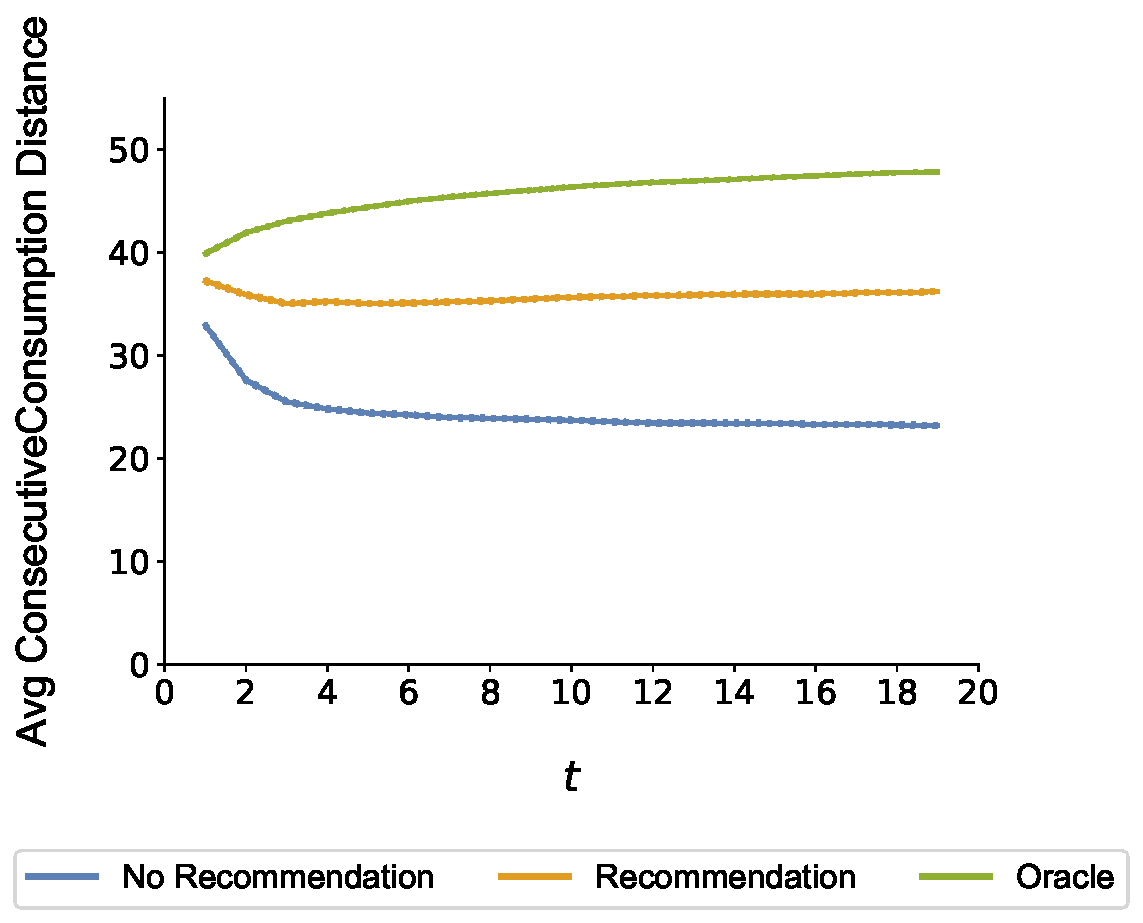
\includegraphics[width=.9\linewidth]{figures/rho_pos_consumption_dist_N_200T_20_overall.pdf}
  \label{fig:sfig1}
\end{subfigure}%
\begin{subfigure}{.5\linewidth}
  \centering
  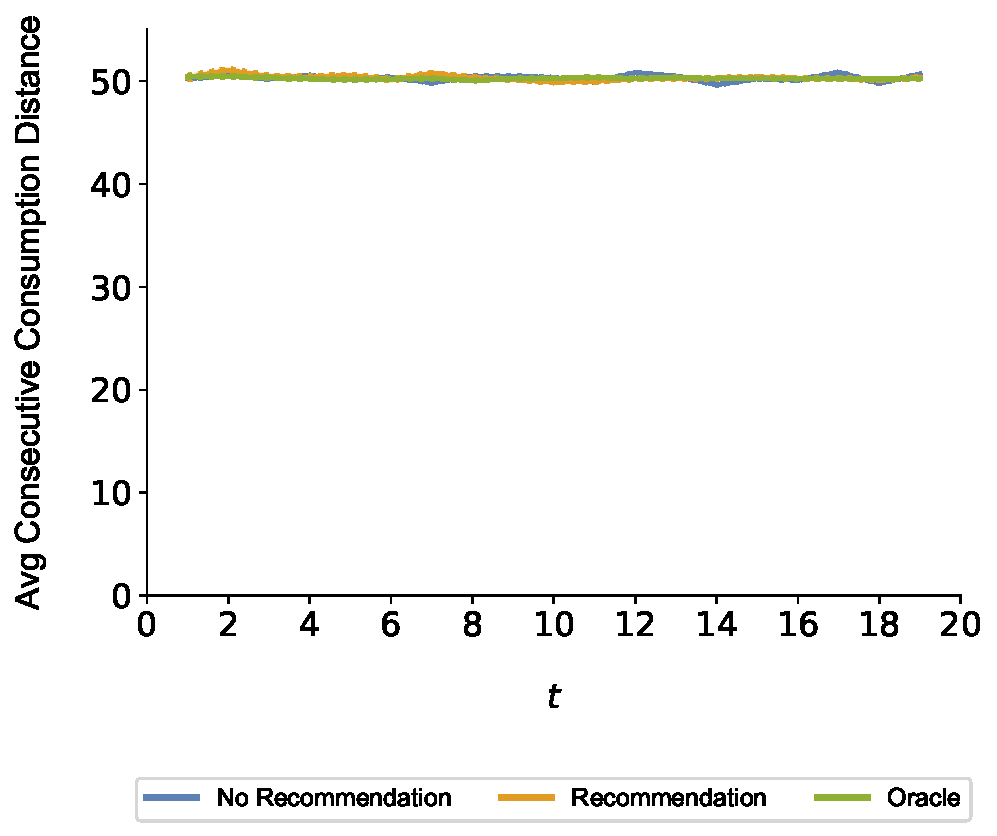
\includegraphics[width=.9\linewidth]{figures/rho_zero_consumption_dist_N_200T_20_overall.pdf}
  \label{fig:sfig2}
\end{subfigure}
\caption*{\scriptsize Notes: The figure shows the consecutive consumption path difference between the no recommendation, recommendation, and oracle regime. The figure on the left displays the average consecutive consumption distance aggregating over simulations where $\rho = 0$ and the figure on the right displays the average consecutive consumption distance aggregating over simulations where $\rho > 0$}
\label{fig:correlation_consumption_path}
\end{figure}

\section{Results}
\subsection{Local Consumption and Filter Bubbles}
We characterize ``filter bubble'' effects in our model as the degree to which users engage in \textit{local consumption}. We define local consumption in terms of the average consumption distance between the items consumed by the users at time $t-1$ and $t$. Thus, in the context of our model, filter bubble effects arise when the average consumption distance decreases over time and, across regimes, when the overall levels are lower for a given recommendation regime compared to another.


\begin{finding}\label{finding_local_consumption}
The impact of recommendation on local consumption:
\begin{enumerate}
\item When $\rho = 0$, there is no difference in consumption distance between the three recommendation regimes.
\item When $\rho > 0$, no recommendation induces more local consumption than both recommendation and oracle regimes. This effect is amplified as $\rho$ increases as well as when users are more risk averse ($\gamma$ increases)
\end{enumerate}
\end{finding}

First, the left panel of Figure \ref{fig:correlation_consumption_path} shows that, when $\rho = 0$, there is no difference in consumption distance between the three regimes. This is due to the fact that when $\rho = 0$, there is no reason that items that are close in the product space should have similar values and so the optimal consumption path does not depend on the similarity of the items. However this also means that users do not learn anything about neighboring products and so there is limited path-dependence in consumption. Not only is there no difference in the levels between the three regimes, but they all have the same, flat, average consumption distance path. This underscores the fact that such concerns about filter bubbles \textit{only} arise in a world where there is correlation between the realized utility of items. If there were no correlation between the realized utilities then there would be no reason for users to consume similar items and thus no narrowing effect, regardless of the information on the true utility of the items that users had.
\par
The left panel of Figure~\ref{fig:correlation_consumption_path} shows that, when $\rho > 0$, both recommendation and no recommendation lead to increasingly local consumption compared to the oracle benchmark case. Further, the average consumption path between periods is \textit{decreasing} for the no recommendation case whereas it is \textit{increasing} for the oracle case. The recommendation regime decreases the degree of local consumption, but not as much as the oracle benchmark. Due to the correlation of values, the oracle consumption path exploits this and leads to the consumption of more similar products than in the case when $\rho = 0$. However, since these spillovers also impact user learning in the no recommendation case, users \textit{over-exploit} this and increasingly consume products similar to good products that they have consumed before. This is further illustrated by Figure 3 in the supplementary material  which shows how the consumption paths in the oracle and no recommendation regimes vary as $\rho$ increases.
\par

Finally, this effect is further amplified as the level of risk aversion, $\gamma$, increases. Figure 4 in the supplementary material shows how drastically the degree of local consumption increases as $\gamma$ increases. This is due to the fact that the spillovers not only affect the mean expected belief about quality but also the degree of uncertainty. Local consumption therefore leads to users having less uncertainty about certain areas of the product space and risk aversion may lead them to increasingly consume nearby products.

In sum, filter bubble effects only arise when there is an inherent correlation between the realized utilities of the items in the product space. When there is a correlation between the realized utilities then filter bubbles can naturally arise due to the nature of how individuals acquire additional information about the remaining items. We have shown that, unless users are provided with additional information to guide their consumption choices, then these information spillovers and user risk-aversion can lead users into filter bubbles. When users consume high valued items, they exploit the underlying correlation across different products' values, stronger for similar products, which leads them to increasingly consume products in narrower and narrower portions of the product space. Risk aversion may lead users into performing local consumption even when they have a low valuation of nearby items just because they know what to expect from the item. Recommendation leads to these effects being mitigated by providing users with additional information on products outside the already explored portions of the product space. Further, if all uncertainty was resolved as in the oracle regime, then such behavior is not present.

\subsection{User Welfare and Product Diversity}
In this section we primarily focus on the impact of recommendation on user welfare and the overall diversity of the items that they consume.
\par 
While in the previous section we looked at the distance between consecutive items, in this section we focus on a diversity measure that considers the entire consumed set of items. The diversity measure we utilize is common in recommender system literature (e.g. \cite{ziegler2005improving}) which is the average normalized pairwise distance between the consumed products:
$$D_i:=\frac{1}{N}\frac{1}{T(T-1)}\sum_{n,m \in C_i^T: n \ne m} d(n,m)$$

\begin{finding}\label{finding_diversity}
The impact of recommendation on product diversity:
\begin{enumerate}
\item When $\rho = 0$, product diversity is the same across all three recommendation regimes;
\item When $\rho > 0$, product diversity decreases across all recommendation regimes but decreases the most in the no recommendation regime. This effect is amplified as $\rho$ increases as well as when users become more risk-averse.
\end{enumerate}
\end{finding}
\par 
Finding~\ref{finding_diversity} summarizes the main results on product diversity. As before, when there is no correlation between valuations, product diversity is the same across different recommendation regimes. The over-exploitation of information spillovers when $\rho > 0$ leads to product diversity being lowest in the no recommendation regime. As a result, this effect gets amplified as $\rho$ increases, which leads to the gap in diversity between the regimes to increase as $\rho$ increases. Figure \ref{fig:diversity_welfare_correlation} shows how diversity varies as $\rho$ increases across the three regimes that we consider.There is a similar increasing diversity gap as $\gamma$, or the level of risk-aversion, increases as can be seen in Figure 4 in the supplementary material. The mechanisms behind these effects have direct parallels to those discussed in the previous section since low average sequential consumption distance directly leads to low diversity.
\par 
We now study how recommendation impacts user welfare in our model. In our model users make consumption decisions that maximize their current period ex-ante utility that depends on their beliefs in that period. Thus, from an ex-ante perspective, they make optimal decisions, but our primary interest is in understanding how the ex-post, or realized, utility varies across regimes and parameter values. We define user's \textit{ex-post} welfare as the average of the realized values, controlling for the effect of $T$:
$$W_i:= \frac{1}{T}\sum_{n \in C_i^T} x_{i,n}$$

\begin{finding}\label{finding_welfare_gap}
The impact of recommendation on consumer welfare is as follows:
\begin{enumerate}
\item Under oracle recommendation, welfare is constant as $\rho$ increases.
\item Under no recommendation, welfare is increasing as $\rho$ increases.
\item Recommendation introduces welfare gains relative to no recommendation, but these gains are decreasing as $\rho$ increases. 
\end{enumerate}
\end{finding}
\par 
Finding~\ref{finding_welfare_gap} states our main findings of the impact of recommendation on ex-post welfare, which are drawn from Figure 1 in the supplementary material. The most interesting observation is that the value of recommendation decreases as $\rho$ decreases. The intuition is clear as recommendation provides users with information that allows them to better guide their decisions and increase welfare. However, as $\rho$ increases users get increasingly more information from consuming items since the realized utility is now more informative about the utility of nearby items. Thus, since consumption decisions themselves reveal information, the information that recommendation reveals provides less value.
\par 
Figure 1 in the appendix shows how diversity and welfare vary across recommendation regimes as the the strength of the common-value component, $\beta$, varies. As expected, when $\beta = 0$, these values are the same. However, as $\beta$ grows the idiosyncratic component of user valuations becomes increasingly less important and the recommendation regime begins to converge to the oracle regime. Indeed, we see that both product diversity and welfare increase under recommendation, whereas under no recommendation we see that there is a decrease in diversity with little changes to consumer welfare. This is intuitive as $\beta$ controls the informativeness of recommendation about user preferences.
\par 
One striking observation is that the decrease in diversity does not appear to be associated with a decline in welfare. Indeed, it appears that the opposite is the case - that low diversity is associated with higher welfare and vice versa. Thus, we next explore the relationship between welfare and diversity.

\addtocounter{figure}{-1}
\begin{figure}[ht]
\caption{Diversity vs. Welfare, \textbf{No Recommendation}}
\begin{subfigure}{.45\textwidth}
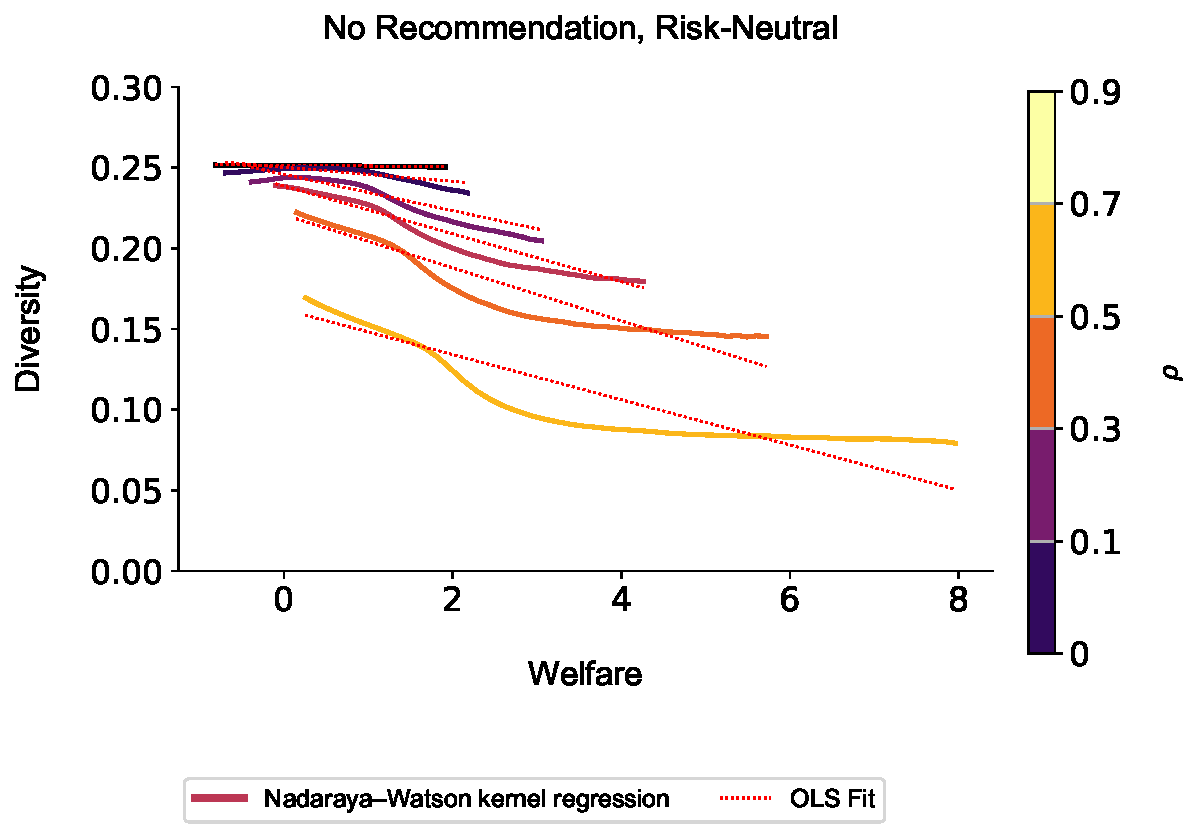
\includegraphics[width=1.0\linewidth]{figures/diversity_welfare_rn_n_200.pdf}
\end{subfigure}
\begin{subfigure}{.45\textwidth}
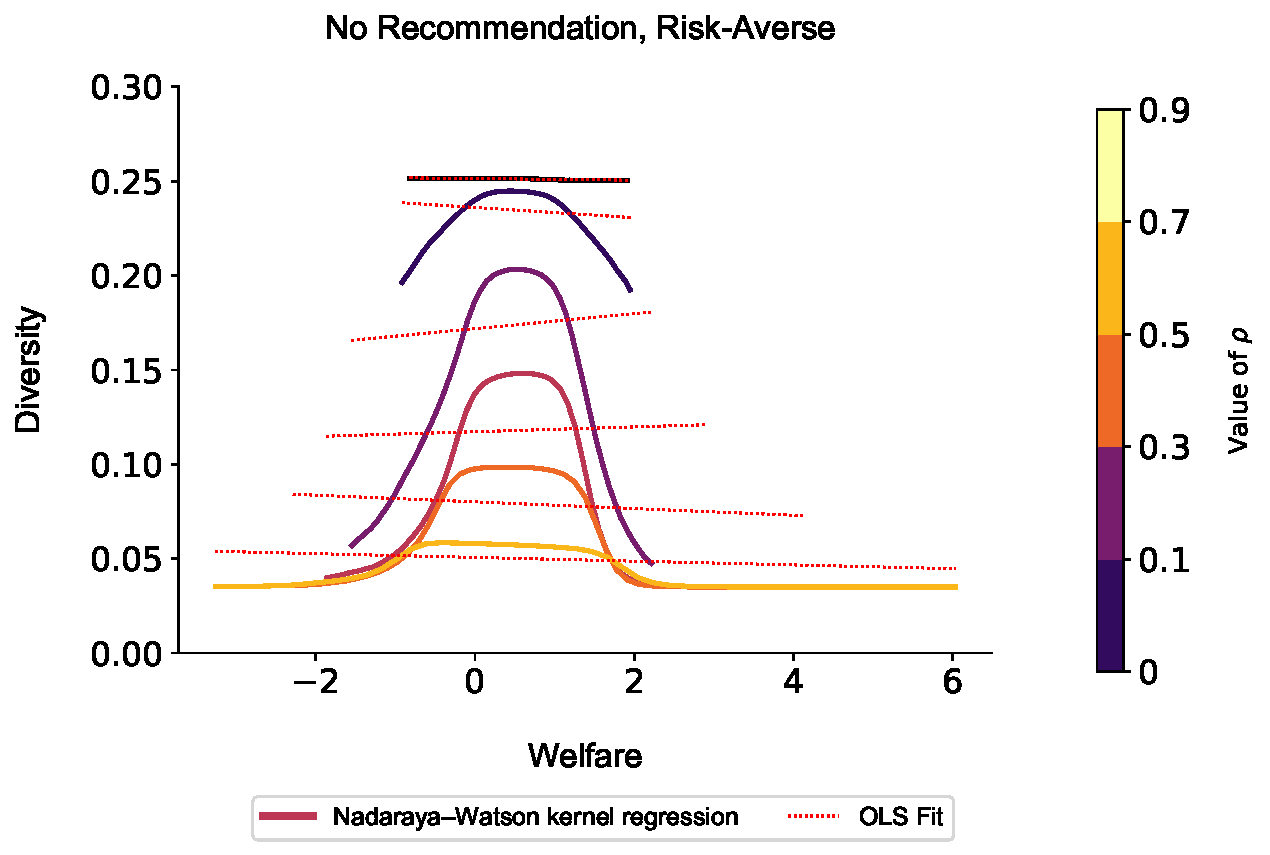
\includegraphics[width=1.0\linewidth]{figures/diversity_welfare_ra_n_200.pdf}
\end{subfigure}\\
\caption*{\scriptsize Notes: The figure plots the relationship between diversity and welfare under the no recommendation regime. The figure on the left displays this relationship for when $\gamma = 0$ and the figure on the right for when $\gamma = 5$.}\label{fig:diversity_welfare_ra}
\end{figure}

\addtocounter{figure}{-1}
\begin{figure}[ht]
\caption{Diversity vs. Welfare, \textbf{Recommendation}}
\begin{subfigure}{.45\textwidth}
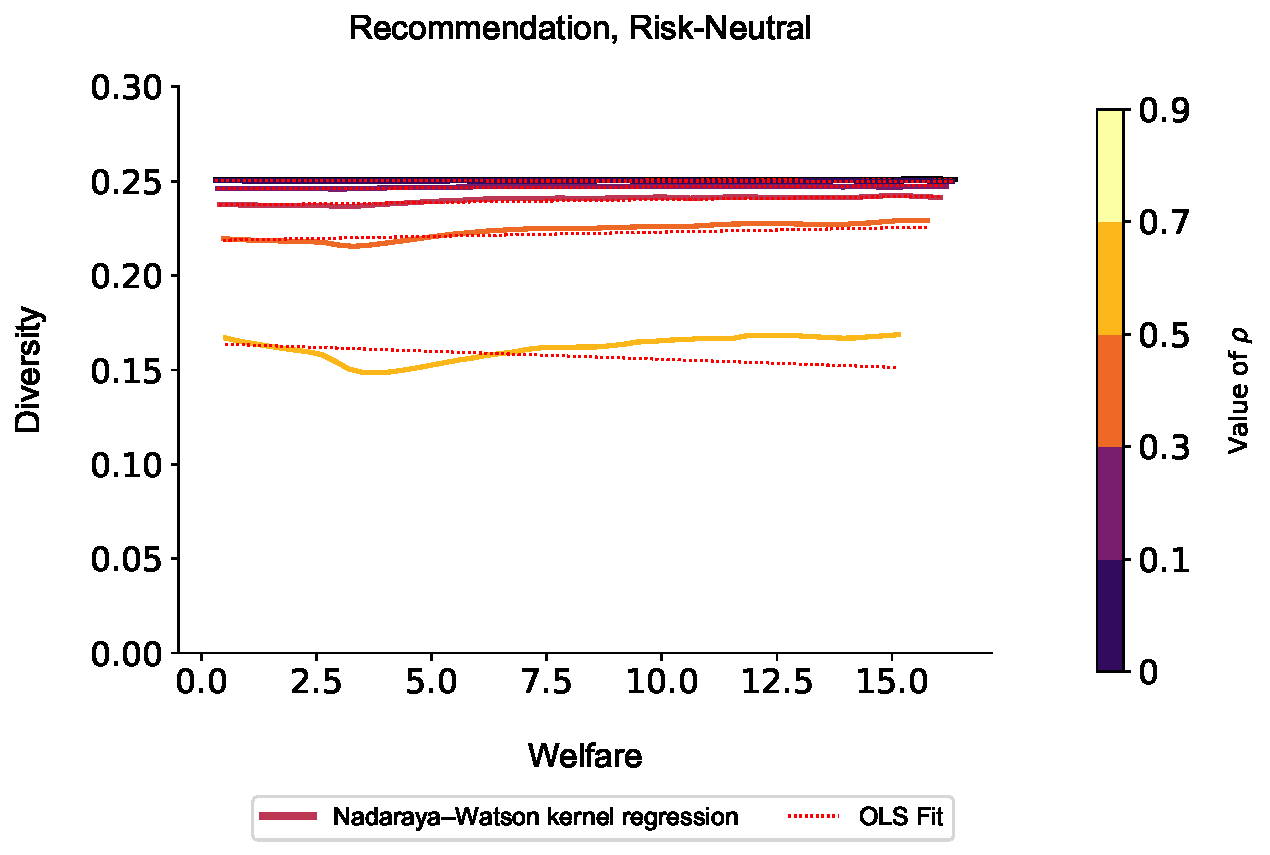
\includegraphics[width=1.0\linewidth]{figures/diversity_welfare_rn_partial_n_200.pdf}
\end{subfigure}
\begin{subfigure}{.45\textwidth}
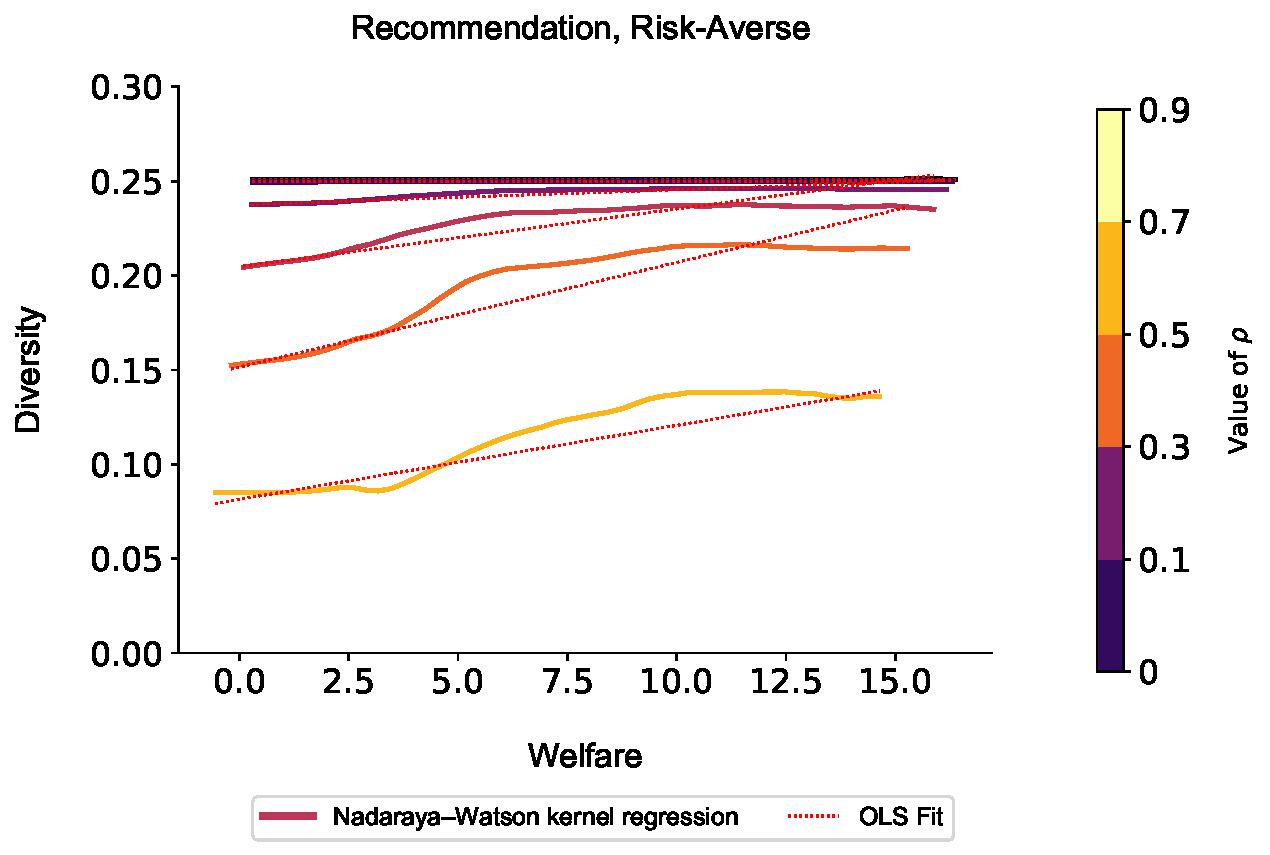
\includegraphics[width=1.0\linewidth]{figures/diversity_welfare_ra_partial_n_200.pdf}
\end{subfigure}\\
\caption*{\scriptsize Notes: The figure plots the relationship between diversity and welfare under the recommendation regime. The figure on the left displays this relationship for when $\gamma = 0$ and the figure on the right for when $\gamma = 5$.}\label{fig:diversity_welfare_ra_partial}
\end{figure}
\addtocounter{figure}{-1}

\begin{finding}\label{finding_diversity_welfare_corr}
In the no recommendation regime, diversity and welfare are:
\begin{enumerate}
\item Negatively correlated when users have no risk-aversion;
\item Uncorrelated when users have high levels of risk-aversion.
\end{enumerate}
In the recommendation regime, diversity and welfare are:
\begin{enumerate}
\item Uncorrelated when users have no risk-aversion;
\item Positively correlated when users have high levels of risk-aversion.
\end{enumerate}
In the oracle regime, diversity and welfare are always uncorrelated.
\end{finding}

Finding~\ref{finding_diversity_welfare_corr} summarizes our findings on the relationship between diversity and welfare. Figure \ref{fig:diversity_welfare_ra} shows how diversity and welfare correlate for the no recommendation case as we vary the degree of risk aversion. When there is no risk-aversion then there is a negative correlation between welfare and diversity. This is since, with no risk-aversion, in a given period a user will select the good that she currently believes has the highest expected value. High product diversity in this case can arise from a user who consumes an item she disliked and updates her beliefs about nearby items negatively. As a result, in the following period she will pick an item far away in the product space from the item that was previously consumed. If instead the user valued highly the item that she had consumed, then she is more likely to pick a nearby item. The information spillovers therefore lead to high product diversity being negatively correlated with welfare.
\par
This only happens since $\gamma = 0$ leads to users only caring about the expected value of the product. However, as we saw in Findings \ref{finding_local_consumption} and \ref{finding_diversity}, increasing $\gamma$ can lead to lower diversity and increasingly local consumption due to the fact that the degree of uncertainty now impacts users' choices. This weakens the negative relationship between diversity and welfare since both negative and positive experiences with a good reduce uncertainty about surrounding items. This leads to the inverted-U shape found in Figure \ref{fig:diversity_welfare_ra} when $\gamma$ is relatively large (e.g $\gamma = 5$) though diversity and welfare are virtually uncorrelated in the data. In the recommendation and oracle regimes, under risk neutrality ($\gamma=0$), welfare and diversity and uncorrelated, while under risk aversion ($\gamma=5$), it is possible to observe in Figure \ref{fig:diversity_welfare_ra_partial} an actual positive relation between diversity and welfare as recommendations are able to reduce uncertainty and facilitate exploration of the product space.

\subsection{User Homogenization}

\begin{figure}[ht]
\caption{Relationship between $\beta$ and Homogeneity, $N = 200$}
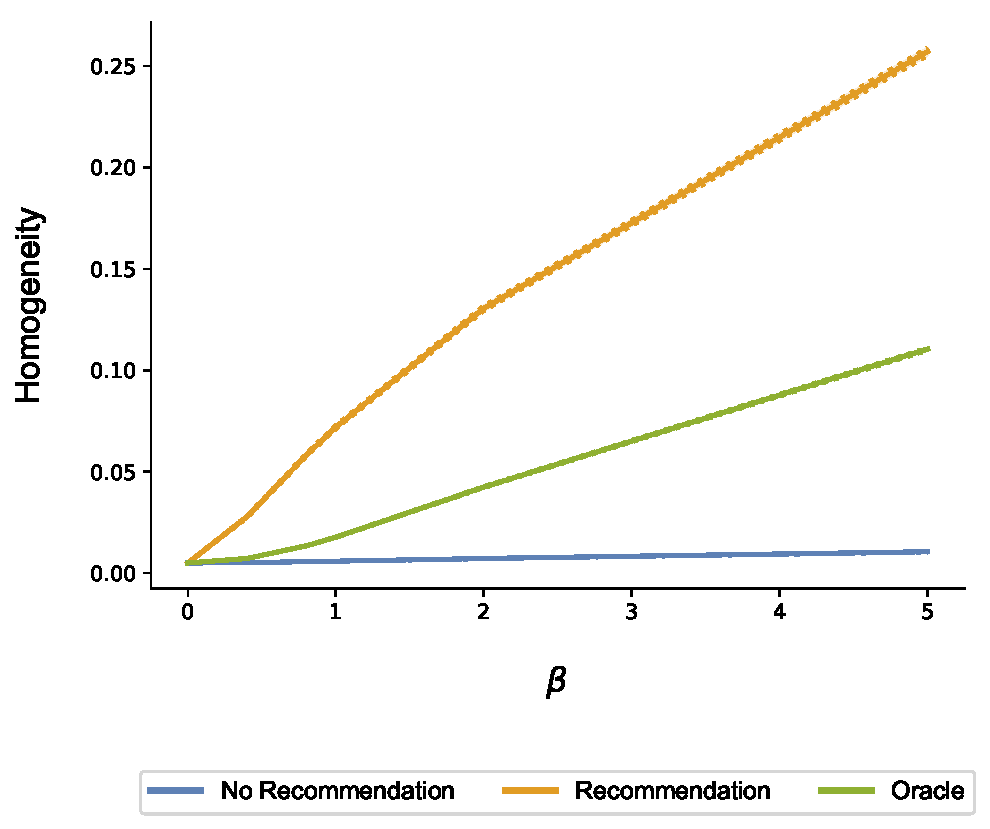
\includegraphics[width=.45\linewidth]{figures/beta_homogeneity_N_200_T_20}\label{fig:beta_homo}
\caption*{\scriptsize Notes: This figure displays the value of the homogeneity measure as we vary the weight of the common value component, $\beta$. Each line represents this plot for a single recommendation regime.}
\end{figure}

In this section, we focus on comparisons across users and investigate how the consumed set of items across users varies across different recommendation regimes and parameter values. In particular we look at the degree of \textit{homogenization} between users. Similar to other papers that study the degree of homogenization in recommender systems (e.g. \cite{chaney2018algorithmic}) we measure homogeneity via the Jaccard index between the consumption sets of users:
\begin{align*}
H:=\frac{1}{|I|(|I|-1)}\sum_{i,j \in I: i \ne j}d_J(C_i^T,C_j^T)
\end{align*}
where $d_J$ denotes the Jaccard index and $H \in [0,1]$.
\begin{finding}\label{finding_homogeneity}
The impact of recommendation on homogeneity is as follows:
\begin{enumerate}
\item Highest under recommendation and lowest under no recommendation;
\item Increasing in $\beta$, or the weight of the common-value component;
\item Decreasing in $\rho$ for partial recommendation, but weakly increasing in $\rho$ for no recommendation.
\end{enumerate}
\end{finding}
Finding~\ref{finding_homogeneity} summarizes our findings on the impact of recommendation on user homogeneity. First, we study how the degree of homogenization varies as we increase $\beta$, the weight of the common value component. As $\beta$ increases we expect that users should become increasingly homogeneous as the realized utilities of the items are now increasingly similar. Figure \ref{fig:beta_homo} confirms that as the weight of the common-value component, $\beta$, increases users consume increasingly similar sets of items. The homogenization effect is strongest under the recommendation regime since the revelation of the common-value component induces users to consume products in similar areas of the product space. As $\beta$ increases, some amount of homogenization is optimal as can be seen from the oracle case. However, since users in the no recommendation regime do not know the common-value component they engage in local consumption in different areas of the product space which leads to less than optimal homogeneity.
\par
We next study how the degree of homogeneity varies as $\rho$ increases. Figure 2 in the supplementary material shows how homogeneity varies as $\rho$ increases across the different recommendation regimes. The most striking finding is that homogeneity decreases as $\rho$ increases in the recommendation regime. As was highlighted in Findings \ref{finding_local_consumption} and \ref{finding_diversity}, the degree of local consumption increases with $\rho$. Even though the revelation of the common-value component induces them to search in similar parts of the product space, their idiosyncratic components induce them to consume products in a more localized area of the product space as $\rho$ increases which leads to a decline in homogeneity.

\section{Recommender System Evaluation}
In this section we discuss how the insights from our model of user decision-making can inform the evaluation and design of recommender systems. The classic approach to recommender system evaluation is to predict user ratings for items and to compare how accurate this prediction is to recorded ratings data, either explicitly given by users or inferred from behavioral data. The recommender system should then recommend the items with the highest predicted ratings \cite{adomavicius2005toward}.
\par
There has been a recent movement away from such evaluation measures due to the observation that accurate recommendations are not necessarily useful recommendations \cite{mcnee2006being}. Our model illustrates a mechanism behind this observation. Consider the domain of movie recommendation and suppose a user has just watched the movie \textit{John Wick} and rated it highly. A recommender system attempting to predict user ratings may then predict that this user is very likely to enjoy the sequel, \textit{John Wick: Chapter Two}, as well. However, the user herself may also have made this inference since the two movies are very similar to each other. Thus, recommending this movie would not be not useful since the recommendation gives the user little information that she did not already know. The key insight is that the recommendation is not useful since \textit{it ignores the inference the user themselves made and their updated beliefs}. The user may watch \textit{John Wick: Chapter Two}, then, even without recommendation, and the value of the recommendation was small.
\par
This intuition implies that recommender systems should collect additional data beyond the type of data that is traditionally recorded. The first and most crucial type of data to collect is individual user \textit{beliefs} about items that they have not yet consumed. As illustrated by our model, these beliefs are what drive the future consumption decisions of users and understanding these beliefs is crucial for determining the value of recommending certain items.\footnote{Additionally, user beliefs contain information that may not have been observed by the recommender that only observes user choices on the platform. There are many sources of information that affect a user's beliefs and choices that are unobservable by recommender systems such as ratings, reviews, and friends. However, this information can be inferred by the platform by collecting both beliefs and consumption choices.} The second type of data that is critical for recommender system designers to collect is how user beliefs change over time and, in particular, not just how individuals value the item they just consumed, but also how it impacts their beliefs about the quality of similar items.\footnote{Characterizing the similarity between items has been an important goal of designing content-based recommendations, though as noted by \cite{winecoff2019users}, how users perceive similarity between items is not always in line with how similarity is computed in content-based recommender systems. Further understanding how users perceive item similarity and, in particular, how this impacts which items users update their beliefs about is an important direction for future work.} The third type of data is the risk-aversion levels of users as our model illustrates that the risk preferences of users are important for understanding what information recommender systems can provide that materially leads users to alter their consumption patterns.
\par 
A natural follow-up question is how this additional data should be utilized in the design of good recommendations. Our model posits that recommendation provides value to users by providing them with information about the true valuation of an item if they were to consume it. Thus, the prediction problem for the recommender becomes predicting what item would the user choose with no recommendation and, correspondingly, what would be the most useful information to provide to the user that would lead her to consume a \textit{better} item than she would without recommendation. This links back to the intuition our model provided for the \textit{John Wick} example whereby collecting user beliefs and measuring how the user updated beliefs about similar goods would lead the recommender to understand that the user would consume \textit{John Wick: Chapter Two}. Our approach would therefore imply that, with this as a starting point, the recommender's problem would be to predict what is the most useful information to give the user leading them to change the item that they eventually consume.
\par 
There have been a number of alternative recommendation evaluation metrics proposed in the literature with the aim of providing more useful recommendations than those provided by accuracy metrics, such as serendipity \cite{kotkov2016survey}, calibration \cite{steck2018calibrated}, coverage \cite{ge2010beyond}, novelty \cite{vargas2011rank}, and many others. Our approach most closely follows the set of proposed serendipity measures which are surveyed in \cite{kotkov2016survey}. As discussed by \cite{maksai2015predicting},  serendipitous recommendations are said to ``have the quality of being both unexpected and useful" which is in line with the primary intuition behind our approach. The primary difference between our proposed approach and those existing in the literature is that ours crucially hinges on understanding user beliefs and the risk-preferences of users. For instance, \cite{vargas2011rank, kaminskas2014measuring} propose unexpectedness metrics that look at the dissimilarity of the proposed recommended items compared to what the recommender already knows the user likes - either via a content-based approach or a collaborative-based approach. This metric depends only on the resulting item-set that the recommender proposes and not necessarily on the user's beliefs or how such a recommendation will change the item that the user consumes. \cite{adamopoulos2015unexpectedness} propose an expected utility approach but use this to measure unexpectedness in terms of deviations from the ``expected consideration set" of a user and do not explicitly incorporate user beliefs.
\par 
Indeed, our approach allows us to give precise definitions for what it means for a recommendation to be \textit{unexpected} and \textit{useful} in the spirit of serendipitous recommendations. Our evaluation measure leads to useful recommendations since it leads users towards better items than they would consume without recommendation. It further results in 	``unexpected" recommendations since it explicitly incorporates user beliefs and thus allows the recommender to understand how ``unexpected" a recommendation would be from the perspective of a user. Thus, a good recommendation provides users with information that leads them to consume an item that they would not have expected to consume without the information from the recommender and that they enjoyed consuming more than the item they would have without recommendation.
% Bibliography
\bibliographystyle{ACM-Reference-Format}
\bibliography{refs}

\end{document}
